\chapter{Le basi di Git}
In questo capitolo vedremo i comandi base per iniziare ad utilizzare Git. Saremo in grado di; inizializzare e configurare un \textit{repository}, gestire il tracciamento di un file, lo stage e il commit, come ignorare alcuni file specifici o famiglie di file tramite pattern specifici, come tornare ad una versione precedente in maniera semplice e veloce, visualizzare lo storico dei commit e come scaricare o caricare i file in un \textit{repository} remoto.
\section{Inizializzare un repository}
Esistono due modi per inizializzare un progetto e sono, o importare un progetto già esistente e caricarlo in Git oppure importare un repository già esistente da un server.
\subsection{Inizializzare un repository da un progetto già esistente }
Se vuoi iniziare a tenere traccia di un progetto già esistente bisogna aprire il CLI, navigare fino alla cartella principale del progetto e lanciare il comando :
\begin{lstlisting}
		git init
\end{lstlisting}
Questo creerà una sottocartella nascosta \textbf{\textit{.git}} che conterrà i file di configurazione del nostro repository per il progetto. A questo punto abbiamo solo lo "scheletro" del nostro repository e ancora nessun file è controllato, nella sua evoluzione, da Git.
Per permettere a Git di seguire l'evoluzione del tuo progetto devi aggiungere i file che vuoi inserire nel repository, tramite il comando :
\begin{lstlisting}
		git add *.c
		git add LICENSE
		git commit -m "inizializzo il progetto"
\end{lstlisting}
Cerchiamo di capire cosa è avvenuto quando abbiamo lanciato questi comandi; con il primo abbiamo aggiunto nell'area di stage tutti i file contenuti nella cartella principale del progetto che abbiano come estensione .c cioè file di codice C.
Con il secondo comando abbiamo inserito nello stage il file \textit{LICENSE} ed in fine con il comando \textit{commit} abbiamo creato una \textit{snapshot} dei file che viene salvata nel DB di Git.
\subsection{Clonare un repository già esistente}
Se vogliamo lavorare su di un progetto che è già stato creato e che risiede su di un server basta usare il comando :
\begin{lstlisting}
	git clone 
\end{lstlisting}
Cosi facendo si scaricano quasi tutti i dati contenuti nel server, compresi tutte le modifiche fatte ai file, così facendo se il progetto sul server dovesse essere danneggiato tutti gli sviluppatori in possesso di un clone hanno una copia che può essere utilizzata per ripristinare i dati, come se avessimo un backup distribuito.
Il comando clone si utilizza nel seguente modo :
\begin{lstlisting}
	git clone [URL]
\end{lstlisting}
In questo modo creerai una cartella con i file del progetto nella cartella dove lancerai il comando.
Scaricando tutti gli ultimi file e impostando una cartella \textbf{.git}. I file scaricati saranno già pronti all'uso e alla modifica del codice. Possiamo inserire il progetto in una nostra cartella nella posizione attuale, aggiungendo un altro parametro cioè il nome dopo l'URL:
\begin{lstlisting}
	git clone [URL] nome_cartella_progetto
\end{lstlisting} 
Il comando è lo stesso del precedente con l'aggiunta di un opzione. si possono utilizzare molti protocolli di comunicazione come ad esempio HTTPS, SSH, git://, ecc. Più in generale sono tutti formati da :  \textbf{\textit{user@server:path/to/repo.git}}.
Quando si scarica un progetto e si vogliono apportare alcune modifiche, i file che sono contenuti sono già tracciati, quindi git rivela le modifiche che hai apportato mentre se crei altri file questi sono nello stato non tracciato, quindi Git non vedrà se sono stati modificati o meno.


\subsection{Registrare i cambiamenti nei repository}
Dopo aver effettuato il clone avrai una copia dell'intero repository in locale, a questo punto puoi iniziare a modificare i file ed effettuare delle \textbf{commit} per tenere aggiornate tutte le modifiche effettuate. In generale i file del tuo progetto possono trovarsi in due stati: tracciati e non tracciati.
I file tracciati sono file della quale git ne è al corrente e questi possono essere in tre condizioni : non modificati, modificati e in staged.
I file non tracciati sono tutto il resto, in pratica tutti i file che sono nella directory di progetto ma che non erano nell'ultima snapshot e che non si trovano nell'area di staging. Quando si effettua un clone tutti i file sono tacciati e non modificati. Quando modifichi i file vengono visti da git come modifica e quindi bisogna effettuare una commit per aggiornare le modifiche.
\begin{figure}[ht]
					\centering
					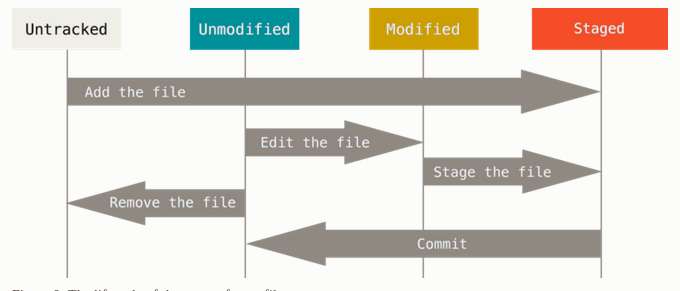
\includegraphics[width=1 \textwidth]{immagini/stato1.png}
					\subitem \caption{stati di un file in git}
					\label{json:imm}
\end{figure}
Questa immagine rappresenta gli stati nella quale si può trovare un file in git.

\subsubsection{Controlare lo stato di un file}
Lo strumento principale per conprendere lo stato dei file è il comando :
\begin{lstlisting}
	git status
\end{lstlisting} 
un tipico status è il segunete :
\begin{figure}[H]
					\centering
					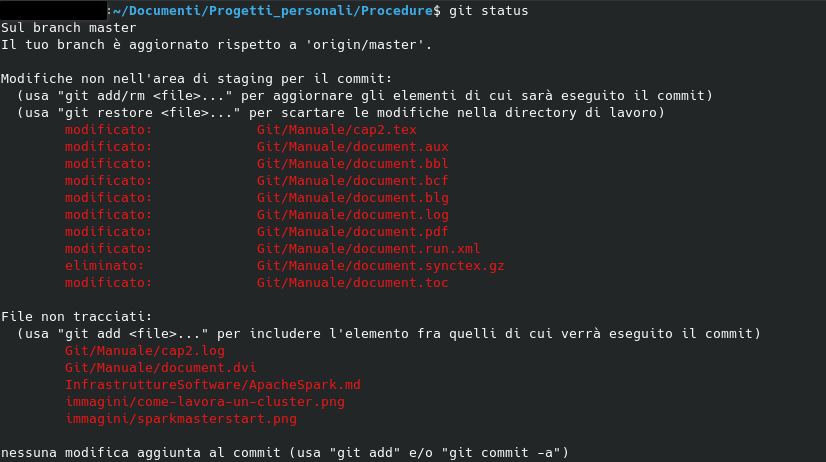
\includegraphics[width=1 \textwidth]{immagini/status.png}
					\subitem \caption{esempio di git status per la modifica di questo manuale}
					\label{json:imm}
\end{figure}
Questo output sta ad indicare che ci sono file che sono stati modificati nello specifico il file cap2.tex, quindi tracciati e poi possiamo notare che ci sono dei file che non sono stati tracciati, che quindi, sono stati creati prima dell'ultimo commit. Un ultima informazione che puoi trarre è il ramo di sviluppo nella quale ti trovi attualmente.
I file non tracciati non verranno aggiunti alle snapshot finche non vengono esplicitamente aggiunti 
\subsubsection{Tracciamento di nuovi file}
Per esplicitare che si vogliono tener traccia di file attualmente non tracciati possimo farlo con il comando : 
\begin{lstlisting}
	git add <nome_file>
\end{lstlisting}
In alternativa possiamo utilizzare il comando :
\begin{lstlisting}
	git add .
\end{lstlisting}
per integrare tutti i file non tracciati all'interno del prossimo commit. Il comando \textbf{git add} accetta percorsi di file o directory, nel caso della directory aggiungerà tutti i file in essa contenuti.
 

